\documentclass{standalone}
\usepackage{tikz}
\usepackage{pgfplots}
\pgfplotsset{width=32cm,height=18cm,compat=1.3}
\pgfplotsset{every tick label/.append style={font=\Huge}}
\usepackage{filecontents}

\usetikzlibrary{patterns}

\definecolor{citrine}{rgb}{0.89, 0.82, 0.04}

\begin{document}
	\centering
		\vspace{1.5em}
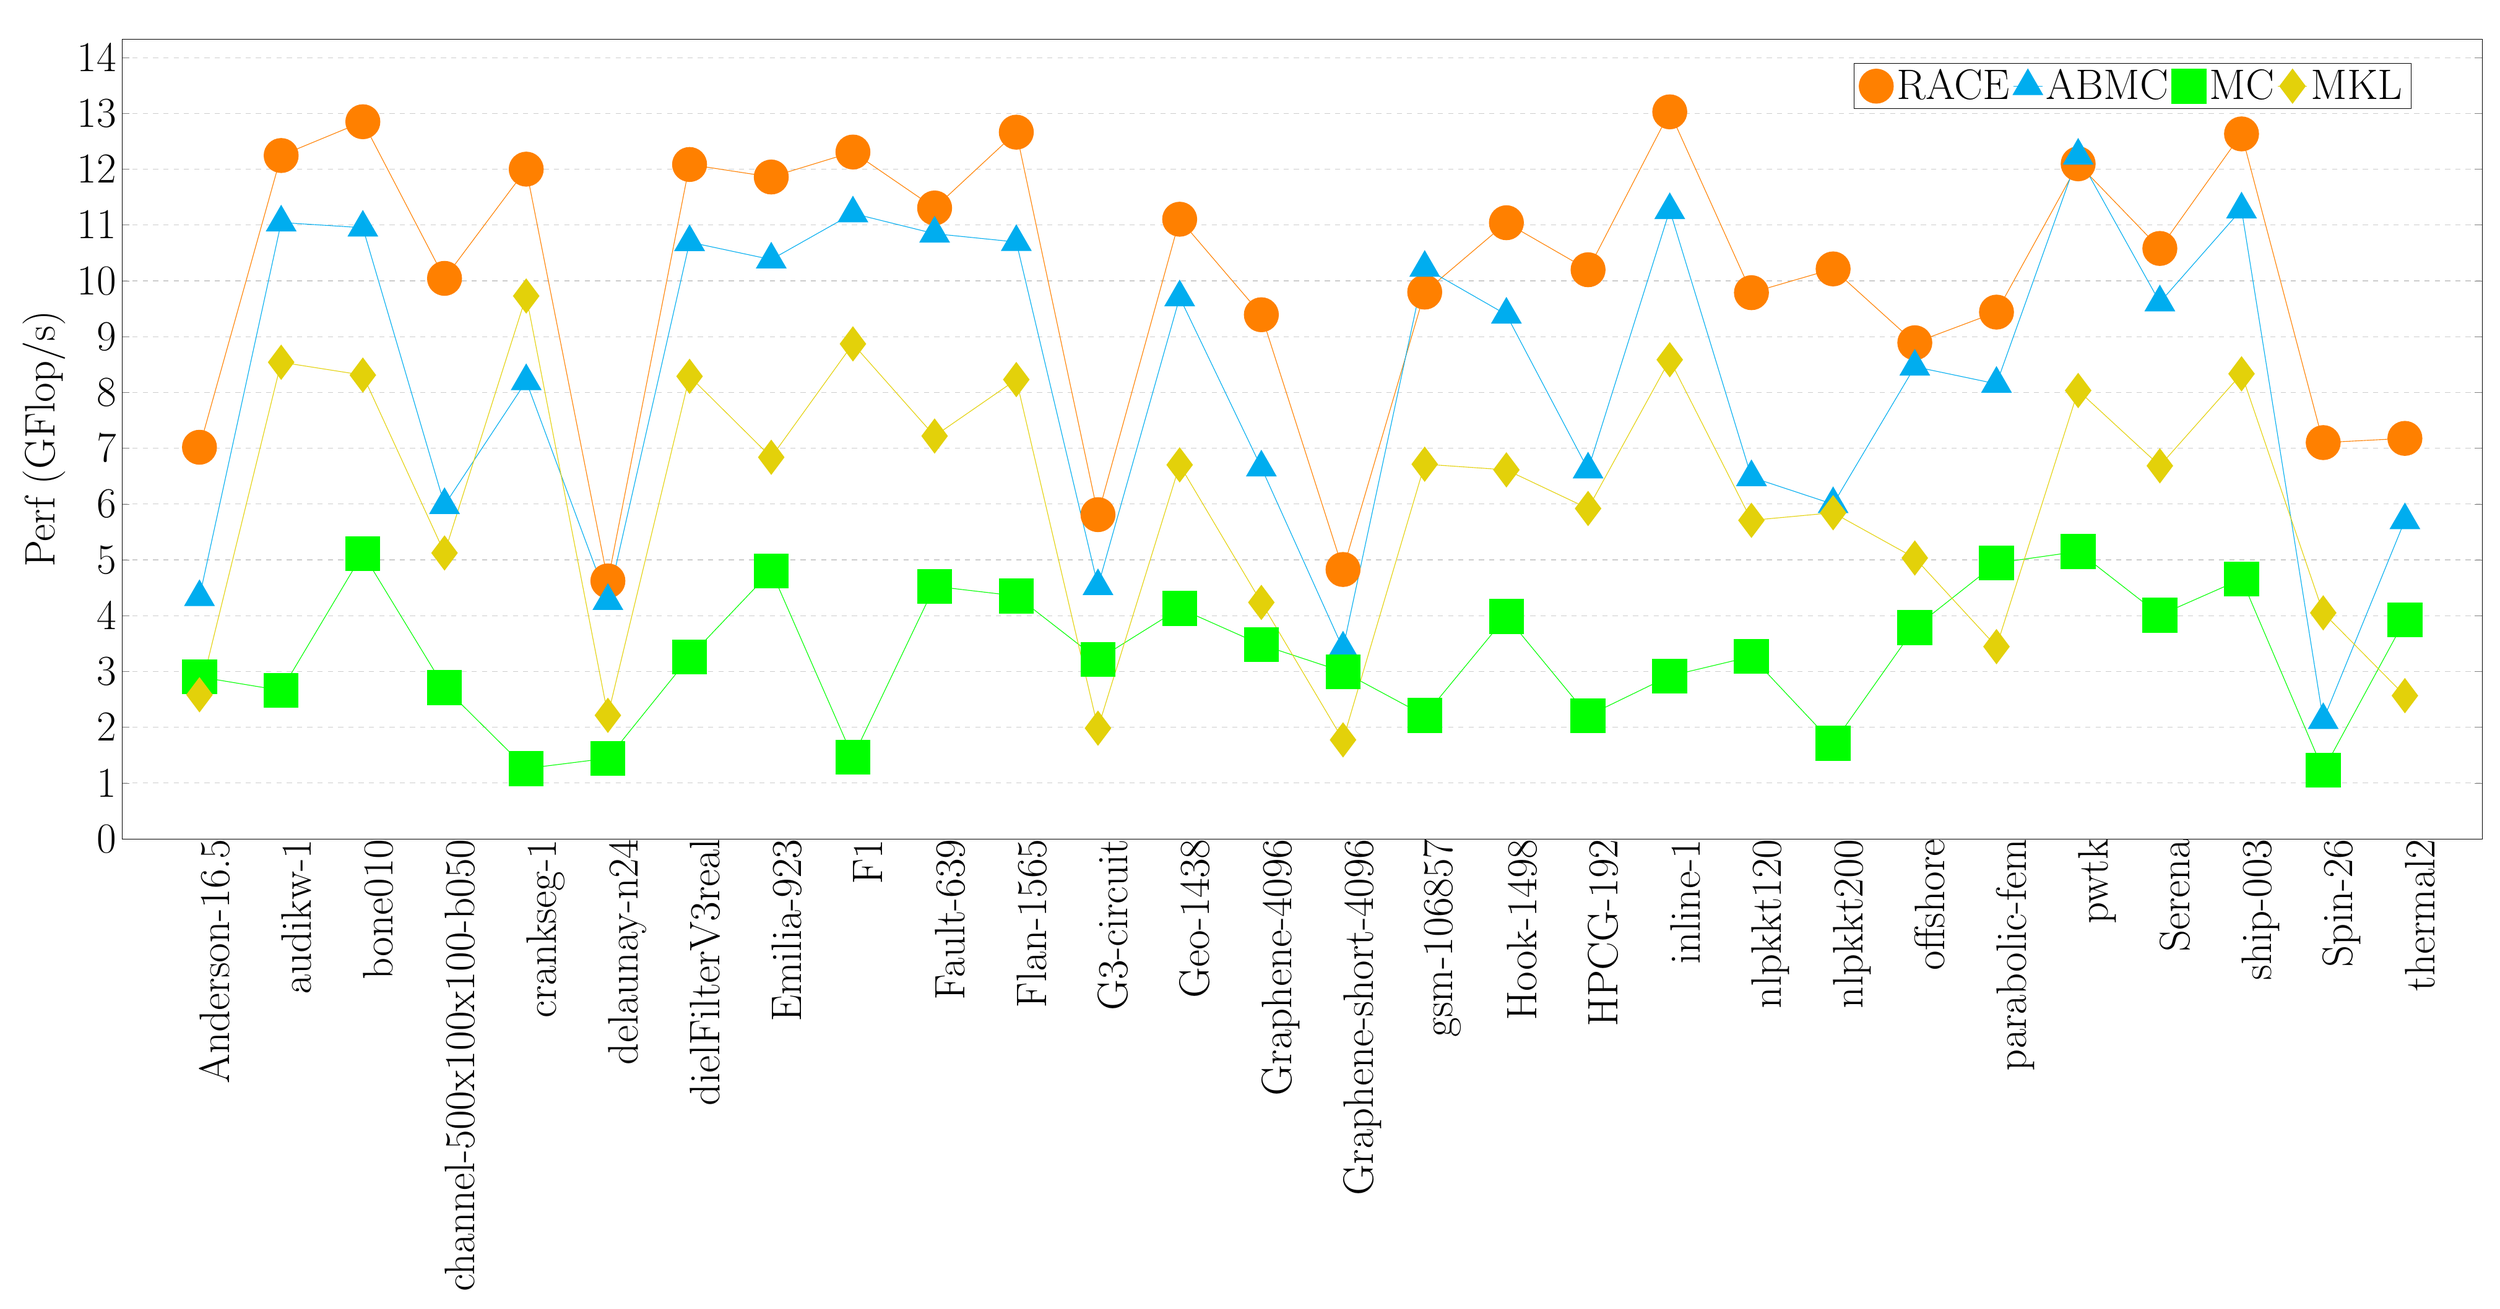
\begin{tikzpicture}
		%	\node at (13.25,15) {\LARGE{}};
			\begin{axis}[
		%	xmin=0.25, xmax=7.25,
			ymin=0, %ymax=3.25,
			xtick={1, 2, 3, 4, 5, 6, 7, 8, 9, 10, 11, 12, 13, 14, 15, 16, 17, 18, 19, 20, 21, 22, 23, 24, 25, 26, 27, 28},
		%	ytick={0,0.5,1,1.5,2,2.5,3},
			xticklabels={Anderson-16.5, audikw-1, bone010, channel-500x100x100-b050, crankseg-1, delaunay-n24, dielFilterV3real, Emilia-923, F1, Fault-639, Flan-1565, G3-circuit, Geo-1438, Graphene-4096, Graphene-short-4096, gsm-106857, Hook-1498, HPCG-192, inline-1, nlpkkt120, nlpkkt200, offshore, parabolic-fem, pwtk, Serena, ship-003, Spin-26, thermal2},
			width  = 50cm,
			height = 18cm,
			major x tick style = transparent,
			%	minor ytick={1, 5, 10, 15, 20, 25, 30 ,35,40},
			grid = minor,	
			%add_bar_commands
			ymajorgrids = true,
			grid style={dashed, gray!40},
			ylabel = {\Huge{Perf (GFlop/s)}},
		%	symbolic x coords={Graphene-2048-2048, Graphene-4096-4096, Spin-24-24-24},
			x tick label style={rotate=90, anchor=north east, inner sep=0mm, font={\Huge}},
			tick label style={font={\Huge}},
			scaled y ticks = false,
			enlarge x limits=0.035,
			legend cell align=left,
			legend style={font=\Huge},
			legend columns=-1,
			legend style={
				%at={(1,1.05)},
				%anchor=south east,
				%column sep=1ex,
				legend pos=north east
			},
			%spl_legend_code
			title= {\Huge\scalebox{1.5}{{}}}
			]

\addplot[mark=*, mark size=10pt, mark options={orange}, draw=orange ] plot coordinates{(1,7.017762) (2,12.245165) (3,12.850634) (4,10.044041) (5,12.001241) (6,4.623104) (7,12.084667) (8,11.860212) (9,12.308086) (10,11.305451) (11,12.663604) (12,5.809891) (13,11.103660) (14,9.392370) (15,4.827286) (16,9.797964) (17,11.040916) (18,10.198226) (19,13.027954) (20,9.787395) (21,10.213585) (22,8.890258) (23,9.439195) (24,12.096590) (25,10.580104) (26,12.632607) (27,7.101122) (28,7.176575)};
\addplot[mark=triangle*, mark size=10pt, mark options={cyan}, draw=cyan ] plot coordinates{(1,4.332372) (2,11.044719) (3,10.951756) (4,5.981806) (5,8.201395) (6,4.2621) (7,10.693218) (8,10.380974) (9,11.207095) (10,10.844468) (11,10.695511) (12,4.527877) (13,9.703719) (14,6.654467) (15,3.409626) (16,10.231921) (17,9.393211) (18,6.618523) (19,11.266553) (20,6.481429) (21,5.997536) (22,8.460706) (23,8.153885) (24,12.241446) (25,9.612898) (26,11.278229) (27,2.128258) (28,5.708837)};
\addplot[mark=square*, mark size=10pt, mark options={green}, draw=green ] plot coordinates{(1,2.902725) (2,2.659737) (3,5.113216) (4,2.711808) (5,1.260992) (6,1.444677) (7,3.260373) (8,4.802827) (9,1.465401) (10,4.525929) (11,4.354064) (12,3.215571) (13,4.130545) (14,3.479720) (15,2.996424) (16,2.210314) (17,3.986207) (18,2.208432) (19,2.918847) (20,3.267880) (21,1.711865) (22,3.785089) (23,4.942191) (24,5.150123) (25,4.010431) (26,4.655164) (27,1.228461) (28,3.925344)};
\addplot[mark=diamond*, mark size=10pt, mark options={citrine}, draw=citrine ] plot coordinates{(1,2.582208) (2,8.540922) (3,8.310591) (4,5.123623) (5,9.728058) (6,2.214071) (7,8.288898) (8,6.838459) (9,8.870003) (10,7.219080) (11,8.230405) (12,1.983922) (13,6.701994) (14,4.237317) (15,1.773905) (16,6.714281) (17,6.612762) (18,5.920205) (19,8.586093) (20,5.708207) (21,5.844054) (22,5.033252) (23,3.445033) (24,8.034666) (25,6.685272) (26,8.333939) (27,4.050526) (28,2.566802)};
	%addplot cmd

	\legend{RACE, ABMC, MC, MKL}

	\end{axis}			
\end{tikzpicture}

\end{document}

